\chapter{Einführung}\label{ch:intro}

Das Smartphone ist heutzutage der stete Begleiter eines Menschen. \enquote{Zwei Drittel der Bevölkerung und nahezu jeder 14- bis 29-Jährige geht darüber ins Netz.} \cite{usage} Auch die Prognose zeigt, das der Absatzmarkt immer weiter steigen wird (Abbildung \ref{fig:prognose_fig}).

\begin{figure}[H]
	\begin{center}
		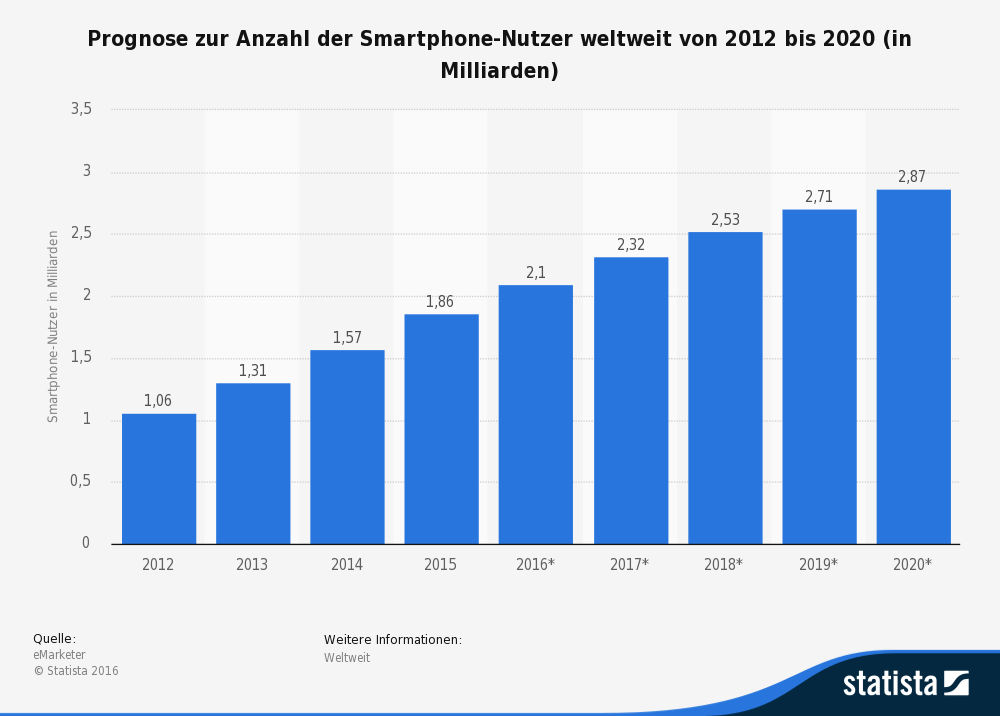
\includegraphics[width=0.86\textwidth]{images/prognose-zur-anzahl-der-smartphone-nutzer-weltweit-bis-2020.png}
		\caption{Prognose zur Anzahl der Smartphone-Nutzer weltweit von 2012 bis 2020 (in Milliarden) \cite{prognose}.}
		\label{fig:prognose_fig}
	\end{center}
\end{figure}

Umso wichtiger ist es, dass die Softwareentwicklung diesen Trend ernst nimmt. Der ehemalige Google-Chef Eric Schmidt sagte bereits 2010: \enquote{Googles Devise heißt jetzt \enquote{Mobile first}}. 
Diese Devise wird von vielen Unternehmen verfolgt und ist der Grund, weswegen in den einzelnen Stores gegenwärtig so viele Apps angeboten werden. Bei Android im Playstore waren im Oktober 2016 ca. 2,4 Millionen Apps \cite{play_store} und bei Apple im App Store ca. 2 Millionen Apps (Stand Juni 2016) verfügbar \cite{app_store}. Neben Googles Android und Apples iOS gibt es noch andere Betriebssysteme, wie beispielsweise Microsofts Windows Phone oder Blackberrys Blackberry OS. Jedoch dominieren die beiden erstgenannten Systeme derzeit den Markt (Abbildung \ref{fig:os_fig}).

\begin{figure}[H]
	\begin{center}
		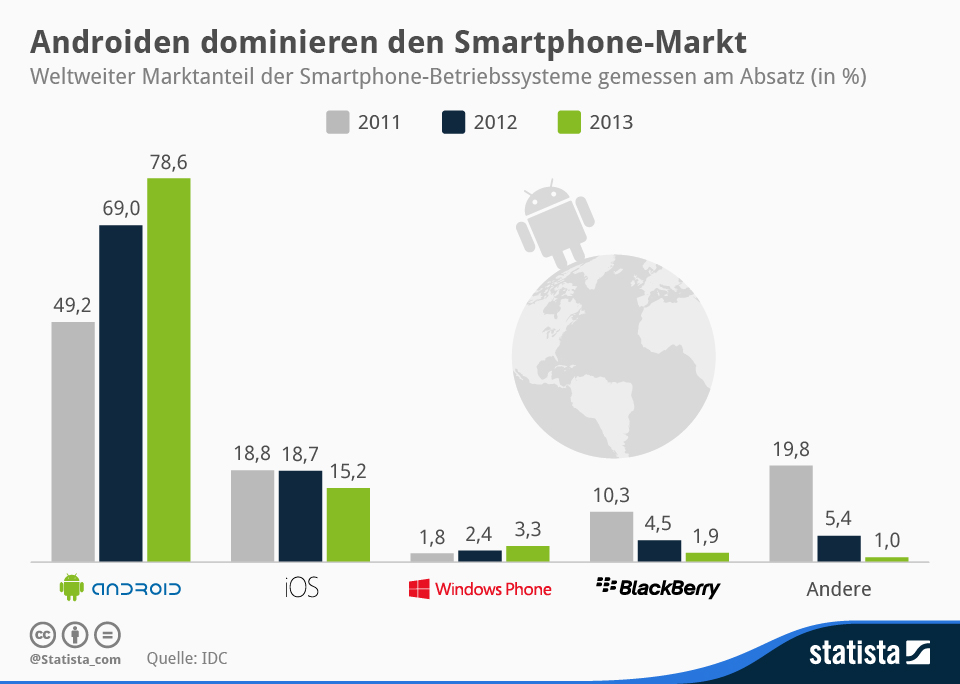
\includegraphics[width=0.86\textwidth]{images/os.jpg}
		\caption{Der weltweite Marktanteil an Smartphone-Betriebssystemen \cite{os}.}
		\label{fig:os_fig}
	\end{center}
\end{figure}

Jede dieser Applikationen wurde einzeln für sich entwickelt und implementiert. Bei jedem Update, zum Beispiel des Systems, müssen alle Anwendungen gewartet und überarbeitet werden, um die volle Funktionalität zu gewährleisten.

Würden einige Applikationen jedoch genauer analysiert werden, wäre das Ergebnis, dass Codepassagen in jeder dieser Anwendungen vorhanden sind, welche einen ähnlichen beziehungsweise denselben Zweck erfüllen. Werden diese Stellen im Programmcode abstrahiert, gibt es die Möglichkeit, diese generieren zu lassen, dafür werden so genannte Code-Generatoren benötigt. 

Im Bereich der Backend-Entwicklung gibt es bereits verschiedene Projekte die sich damit befassen. Ein Beispiel wäre der \textit{CRUD Admin Generator} \cite{generators}. Die Hochschule für angewandte Wissenschaften Würzburg-Schweinfurt entwickelt  unter der Leitung von Prof. Dr. Peter Braun auch einen Code-Generator unter dem Namen \ac{gemara}. Mit Hilfe solcher Generatoren für den Bereich Mobiler Applikationen könnte der Entwicklungs- und Wartungsaufwand reduziert werden. 

Führt ein Systemupdate dazu, dass die Implementierung verschiedener Anforderungen nicht länger funktionsfähig ist, muss dies nur einmalig an der entsprechenden Stelle im Code-Generator geändert werden und nicht in jeder Applikation einzeln. 

\section{Motivation}\label{sec:motivation}
Im Rahmen des Projektes \ac{gemara} gab es bereits Arbeiten, welche sich mit dem Thema der Generierung von \textit{Android Activities} beschäftigt. Die dabei entstandenen Lösungen resultieren darin, dass das Generieren von \textit{Activities} zu Problemen führt. Deshalb behandelt diese Ausarbeitung das Erzeugen von sogenannten Komponenten und nicht kompletter \textit{Activity}.

Eine Komponente ist im Wesentlichen eine kleine Anwendung für sich, welche nur eine einzige Aufgabe erfüllt. Dies könnte zum Beispiel das Anzeigen eines Dozenten in einer Campus-Applikation sein.
Aus den erzeugten Komponenten kann eine Art Bausatz entstehen, mit dessen Hilfe der Entwickler seine Applikation zusammen bauen kann. Dabei wird ihm freie Wahl gelassen, wie der Aufbau seiner Anwendung aussieht. Er bedient sich nur an gegebener Stelle an den Komponenten. Dadurch reduziert sich der Entwicklungsaufwand für ihn.

Bewegen wir uns in der Domain einer Hochschule, kann eine Bibliothek mit den erzeugten Komponenten allen Studierenden zur Verfügung gestellt werden. Dadurch wäre jeder Studierende in der Lage eine persönliche Campus-Applikation zu entwickeln. Durch die einzelnen Komponenten kann dann sichergestellt werden, dass grundsätzliche Funktionalität bereits gewährleistet ist.

\section{Zielsetzung}\label{sec:target}
Ziel dieser Ausarbeitung ist es, dass der Leser einen grundsätzlichen Überblick für die Entwicklung von Android Applikationen beziehungsweise Android-Bibliotheken vermittelt bekommt. Weiterhin soll das Wissen des Lesers über Datenkommunikation mittels \textit{\acf{rest}} vertieft werden. Hierbei wird der Schwerpunkt auf das \textit{Hypermedia-Prinzip} gelegt. 

Neben diesen spezifischen Anforderungen soll ein Verständnis der Implementierung von Generatoren entstehen. Dafür muss der Entwickler entscheiden können, was von der Implementierung als statischer Code angesehen werden kann und welcher generisch ist. Dieses Verständnis ist wichtig, um die Komplexität der Generatoren zu reduzieren. Da die statischen Anteile jedes Mal identisch sind.
Auch soll auf die Frage eingegangen werden, ob das \textit{\ac{ui}}, welches ebenfalls generiert wird, auch generisch gestaltet werden kann. Das bedeutet, dass nicht nur Informationen, welche angezeigt werden sollen, beschrieben werden, sondern auch, wie diese angezeigt werden sollen.

Wenn es möglich ist, dass das \textit{\ac{ui}} als Teil der \textit{domänenspezifischen Sprache (DSL)} beschrieben werden kann, so hat der Nutzer des entsprechenden Generators die Freiheit, selbst zu entscheiden, ob zum Beispiel in seiner Campus-App bei der Liste aller Dozenten das Profilbild links oder rechts angezeigt werden soll.

\section{Aufbau der Arbeit}\label{sec:structure}
Diese Ausarbeitung ist in sieben Kapitel unterteilt. In der Einführung wird zu Beginn auf den Stellenwert von Android Applikationen eingegangen. Im Kapitel Motivation wird die Problemstellung angerissen und zur Zielsetzung hingeführt. Mit dem Aufbau der Arbeit wird das Kapitel abgeschlossen.

Das zweite Kapitel befasst sich mit den Grundlagen. Hier soll der Leser noch einmal seinen Kenntnisstand über \textit{\acf{rest}} auffrischen und die Bedeutung von \textit{\acf{hateoas}} verstehen können. Neben dem Bereich der Netzwerkkommunikation wird außerdem noch der Bereich Android angeschnitten. Hier liegt der Schwerpunkt in der Entwicklung von Applikationen und \textit{CustomViews}. Dabei werden die einzelnen Schritte aufgezeigt, um diese Komponenten zu erstellen und zu benutzen. Der letzte Teil in den Grundlagen befasst sich mit Software-Generatoren. Der Leser erhält einen Einblick drüber, was eine \textit{\acf{dsl}} ist und in welche zwei generelle Arten diese eingeteilt werden. Im Anschluss folgt die Vorstellung des Projekts \acf{gemara}. 

Das dritte Kapitel behandelt die Problemstellung. Dabei wird die Referenzanwendung vorgestellt. Diese Vorstellung inkludiert sowohl das Backend als auch die Android Applikation. Es enthält weitergehend die Generierung des Backends mit Hilfe von \ac{gemara} und das Aussehen des daraus resultierenden \ac{api}. 
Anschließend wird die Android Anwendung analysiert. Dabei wird sowohl der Aufbau der Applikation als auch die einzelnen \textit{Views} betrachtet. Die Analyse des Aufbaus soll eine Einteilung in einen generischen sowie spezifischen Quellcode ermöglichen. Bei der Betrachtung der \textit{Views} sollen Gemeinsamkeiten im Aufbau und Design offenbart werden, so dass diese mit einer \textit{\ac{dsl}} modellierbar sind. Zum Abschluss wird das \textit{Meta-Modell} vorgestellt. Es wird auf die Anforderungen an dieses eingegangen und anschließend zwei weitere Modelle vorgestellt. Ein reines Android Modell und die Erweiterung des vorhandenen Enfield-Modells. Das \textit{Meta-Modell} wird dahingehend untersucht, um herauszufinden, welche Daten das \textit{Meta-Modell} benötigt. Bei dem analysieren der einzelnen \textit{Views} wird ein Augenmerk auf den Programmablauf und die Aktionen bei Klick gelegt. Anschließend folgt die Vorstellung des Aufbaus der \textit{View-Meta-Modelle}. Bei jeder \textit{View} wird auf deren Besonderheiten und Möglichkeiten eingegangen. Neben den \textit{View-spezifischen} Daten wird auch noch aufgezeigt, welche Dateien allgemein benötigt werden und wo deren Platzierung im vorgegebenen Modell ist.

Im Kapitel Lösung wird der in dieser Arbeit entwickelte Software-Generator \textit{Welling} vorgestellt.
Zunächst erfolgt die Vorstellung des \textit{Java \acf{api} JavaPoet} zur Generierung von Java-Klassen. Anschießend wird beschrieben, wie andere Datei-Typen generiert werden können. Es wird gezeigt, welche Features unterstützt werden müssen. Nachfolgend wird der Aufbau des Generators vorgestellt. Es wird auf die einzelnen Bereiche eingegangen und deren Aufgabe sowie Funktionsweise erklärt. Abgeschlossen wird das Kapitel mit einer Anleitung, wie die generierte Applikation gebaut und ausgeführt werden kann.

Das fünfte Kapitel, Evaluierung anhand einer Beispielanwendung, ist in drei Bereiche eingeteilt. Zunächst wird die Beispielanwendung vorgestellt. Anschließend wird auf die Erstellung und Nutzung des \textit{Meta-Modells} eingegangen, wobei hier auch Einschränkungen durch dieses aufgezeigt werden. Der letzte Bereich befasst sich mit dem Zeitaufwand und der Komplexität der Entwicklung, Wartung sowie Nutzung des Generators. Auch wird die Komplexität der erzeugten Applikation kritisch bewertet.

Im letzten Kapitel, Zusammenfassung, wird die Arbeit reflektiert und zusätzliche Erweiterungen und Ergänzungen an \textit{Meta-Modell} und Software-Generator dargestellt.